% Options for packages loaded elsewhere
% Options for packages loaded elsewhere
\PassOptionsToPackage{unicode}{hyperref}
\PassOptionsToPackage{hyphens}{url}
\PassOptionsToPackage{dvipsnames,svgnames,x11names}{xcolor}
%
\documentclass[
  10pt,
]{article}
\usepackage{xcolor}
\usepackage[top=0.32in,bottom=0.32in,left=0.583in,right=0.583in]{geometry}
\usepackage{amsmath,amssymb}
\setcounter{secnumdepth}{-\maxdimen} % remove section numbering
\usepackage{iftex}
\ifPDFTeX
  \usepackage[T1]{fontenc}
  \usepackage[utf8]{inputenc}
  \usepackage{textcomp} % provide euro and other symbols
\else % if luatex or xetex
  \usepackage{unicode-math} % this also loads fontspec
  \defaultfontfeatures{Scale=MatchLowercase}
  \defaultfontfeatures[\rmfamily]{Ligatures=TeX,Scale=1}
\fi
\usepackage{lmodern}
\ifPDFTeX\else
  % xetex/luatex font selection
\fi
% Use upquote if available, for straight quotes in verbatim environments
\IfFileExists{upquote.sty}{\usepackage{upquote}}{}
\IfFileExists{microtype.sty}{% use microtype if available
  \usepackage[]{microtype}
  \UseMicrotypeSet[protrusion]{basicmath} % disable protrusion for tt fonts
}{}
\makeatletter
\@ifundefined{KOMAClassName}{% if non-KOMA class
  \IfFileExists{parskip.sty}{%
    \usepackage{parskip}
  }{% else
    \setlength{\parindent}{0pt}
    \setlength{\parskip}{6pt plus 2pt minus 1pt}}
}{% if KOMA class
  \KOMAoptions{parskip=half}}
\makeatother
% Make \paragraph and \subparagraph free-standing
\makeatletter
\ifx\paragraph\undefined\else
  \let\oldparagraph\paragraph
  \renewcommand{\paragraph}{
    \@ifstar
      \xxxParagraphStar
      \xxxParagraphNoStar
  }
  \newcommand{\xxxParagraphStar}[1]{\oldparagraph*{#1}\mbox{}}
  \newcommand{\xxxParagraphNoStar}[1]{\oldparagraph{#1}\mbox{}}
\fi
\ifx\subparagraph\undefined\else
  \let\oldsubparagraph\subparagraph
  \renewcommand{\subparagraph}{
    \@ifstar
      \xxxSubParagraphStar
      \xxxSubParagraphNoStar
  }
  \newcommand{\xxxSubParagraphStar}[1]{\oldsubparagraph*{#1}\mbox{}}
  \newcommand{\xxxSubParagraphNoStar}[1]{\oldsubparagraph{#1}\mbox{}}
\fi
\makeatother


\usepackage{longtable,booktabs,array}
\newcounter{none} % for unnumbered tables
\usepackage{calc} % for calculating minipage widths
% Correct order of tables after \paragraph or \subparagraph
\usepackage{etoolbox}
\makeatletter
\patchcmd\longtable{\par}{\if@noskipsec\mbox{}\fi\par}{}{}
\makeatother
% Allow footnotes in longtable head/foot
\IfFileExists{footnotehyper.sty}{\usepackage{footnotehyper}}{\usepackage{footnote}}
\makesavenoteenv{longtable}
\usepackage{graphicx}
\makeatletter
\newsavebox\pandoc@box
\newcommand*\pandocbounded[1]{% scales image to fit in text height/width
  \sbox\pandoc@box{#1}%
  \Gscale@div\@tempa{\textheight}{\dimexpr\ht\pandoc@box+\dp\pandoc@box\relax}%
  \Gscale@div\@tempb{\linewidth}{\wd\pandoc@box}%
  \ifdim\@tempb\p@<\@tempa\p@\let\@tempa\@tempb\fi% select the smaller of both
  \ifdim\@tempa\p@<\p@\scalebox{\@tempa}{\usebox\pandoc@box}%
  \else\usebox{\pandoc@box}%
  \fi%
}
% Set default figure placement to htbp
\def\fps@figure{htbp}
\makeatother





\setlength{\emergencystretch}{3em} % prevent overfull lines

\providecommand{\tightlist}{%
  \setlength{\itemsep}{0pt}\setlength{\parskip}{0pt}}



 


% =====================================================================
%  _brief-style.tex  ·  Design system for the one-page policy brief
%  Tokens below were extracted from the source Claude Design HTML.
%  Edit here to restyle ALL briefs. Included via the .qmd YAML.
% =====================================================================

% ---- Colours (exact hex from source) --------------------------------
\definecolor{ink}{HTML}{1D2620}        % headings, title, pull quote
\definecolor{body}{HTML}{33352C}       % main body paragraphs
\definecolor{accentred}{HTML}{641111}  % POLICY BRIEF, links, fig title, chart
\definecolor{boxred}{HTML}{8C2826}     % bottom-line box fill
\definecolor{labeltan}{HTML}{E6B894}   % "BOTTOM LINE" label on the box
\definecolor{boxtext}{HTML}{EEF1EA}    % bottom-line body text (off-white)
\definecolor{rosebg}{HTML}{F7EEED}     % pull-quote background
\definecolor{roseborder}{HTML}{E6D2D0} % pull-quote border
\definecolor{muted}{HTML}{50534A}      % column bodies, fig source
\definecolor{cite}{HTML}{6E6D61}       % citation line
\definecolor{faint}{HTML}{9A978A}      % footer
\definecolor{warmrule}{HTML}{D8D2C2}   % thin warm-grey dividers
\definecolor{paper}{HTML}{FAF8F1}      % warm page background

% \pagecolor{paper}                    % uncomment for warm off-white background

% ---- Fonts ----------------------------------------------------------
% Source: Source Sans 3 / Source Serif 4. The CTAN packages below provide
% Adobe Source Sans/Serif (same typefaces); TinyTeX auto-installs them.
\usepackage[T1]{fontenc}
\usepackage[default]{sourcesanspro}
\usepackage{sourceserifpro}
\renewcommand{\familydefault}{\sfdefault}

% ---- Page -----------------------------------------------------------
\pagestyle{empty}
\setlength{\parindent}{0pt}
\setlength{\parskip}{2pt}
% default body size/colour (12.5px -> 9.4pt, line-height 1.45)
\AtBeginDocument{\color{body}\fontsize{9.4pt}{13.6pt}\selectfont}

% ---- Packages -------------------------------------------------------
\usepackage{microtype}
\usepackage{soul}
\setul{2pt}{.5pt}
\usepackage{tcolorbox}
\tcbuselibrary{skins}

% column regions — same size as body
\newcommand{\colsize}{\color{muted}\fontsize{9.4pt}{13.6pt}\selectfont}
% implications columns — smaller, matches target design
\newcommand{\impcolsize}{\color{muted}\fontsize{8.25pt}{11.7pt}\selectfont}

% =====================================================================
%  MACROS
% =====================================================================

% --- Masthead: {logo}{right label} + 3px ink rule --------------------
\newcommand{\briefheader}[2]{%
  \noindent
  \begin{minipage}[c]{0.62\linewidth}\raggedright\color{ink} #1\end{minipage}\hfill
  \begin{minipage}[c]{0.36\linewidth}\raggedleft
    \fontsize{8.25pt}{10pt}\selectfont\bfseries\color{accentred}%
    \textls[200]{\MakeUppercase{#2}}%
  \end{minipage}

  \vspace{2pt}
  \noindent\textcolor{ink}{\rule{\linewidth}{2.2pt}}
  \vspace{-3pt}
}

% --- Title + citation (citation has a thin warm divider beneath) ------
\newcommand{\brieftitle}[1]{%
  {\color{ink}\fontsize{18pt}{19.5pt}\selectfont\bfseries\textls[-12]{#1}\par}\vspace{3pt}}
\newcommand{\briefcitation}[1]{%
  {\color{cite}\fontsize{9.4pt}{12pt}\selectfont #1\par}\vspace{3pt}%
  \noindent\textcolor{warmrule}{\rule{\linewidth}{0.7pt}}}

% --- Section heads (13px 900 uppercase, ls 0.02em) -------------------
\newcommand{\sectionhead}[1]{%
  \vspace{2pt}{\color{ink}\bfseries\fontsize{9.75pt}{12pt}\selectfont
  \textls[20]{\MakeUppercase{#1}}\par}\vspace{1pt}}
% with a 2px ink rule beneath (IMPLICATIONS)
\newcommand{\sectionheadruled}[1]{%
  \vspace{5pt}{\color{ink}\bfseries\fontsize{9.75pt}{12pt}\selectfont
  \textls[20]{\MakeUppercase{#1}}\par}%
  \vspace{3pt}\noindent\textcolor{ink}{\rule{\linewidth}{1.5pt}}\vspace{3pt}}

% --- Sub-heads -------------------------------------------------------
% small uppercase (11px, ls 0.05em) — WHY COMPLIANCE MATTERS
\newcommand{\subhead}[1]{%
  {\color{ink}\bfseries\fontsize{8.25pt}{10pt}\selectfont
  \textls[50]{\MakeUppercase{#1}}\par}\vspace{2pt}}
% 2px ink top rule + title-case bold heading — Funding / Oversight
\newcommand{\colhead}[1]{%
  \noindent\textcolor{ink}{\rule{\linewidth}{1.5pt}}\par\vspace{2pt}%
  {\color{ink}\bfseries\fontsize{9pt}{11pt}\selectfont #1\par}\vspace{1pt}}

% --- Figure title ----------------------------------------------------
\newcommand{\figtitle}[2]{%
  {\bfseries\color{accentred}\fontsize{7.1pt}{9pt}\selectfont\textls[40]{\MakeUppercase{#1}}}%
  \ {\color{muted}\fontsize{7.1pt}{9pt}\selectfont #2}\par\vspace{4pt}}

% --- Inline links (underlined accent red, wraps across lines) --------
\newcommand{\brieflink}[1]{{\color{accentred}\ul{#1}}}
\newcommand{\quotelink}[1]{{\bfseries\color{accentred}\ul{#1}}}

% --- Footer (warm divider + faint text, pinned to bottom) ------------
\newcommand{\brieffooter}[1]{%
  \par\vfill
  \noindent\textcolor{warmrule}{\rule{\linewidth}{0.7pt}}\par\vspace{5pt}%
  {\color{faint}\fontsize{7.1pt}{9.5pt}\selectfont #1\par}}

% =====================================================================
%  COLOURED BOXES (border-radius 6px -> arc=4pt)
% =====================================================================

% --- Bottom-line box -------------------------------------------------
\newtcolorbox{bottomline}{%
  enhanced, arc=4pt, outer arc=4pt, boxrule=0pt,
  colback=boxred, coltext=boxtext,
  left=7pt, right=7pt, top=7pt, bottom=7pt,
  before upper={{\fontsize{7.1pt}{9pt}\selectfont\textls[120]{%
    \bfseries\textcolor{labeltan}{BOTTOM LINE}}}\par\vspace{3pt}%
    \fontsize{9.4pt}{13.6pt}\selectfont}}

% --- Pull-quote box (serif, 13.5px -> 10.1pt, with rose border) ------
\newtcolorbox{pullquote}{%
  enhanced, arc=4pt, outer arc=4pt, boxrule=0.7pt,
  colback=rosebg, colframe=roseborder, coltext=ink,
  left=7pt, right=7pt, top=11pt, bottom=12pt,
  fontupper={\rmfamily\fontsize{11.5pt}{16.5pt}\selectfont}}
\makeatletter
\@ifpackageloaded{caption}{}{\usepackage{caption}}
\AtBeginDocument{%
\ifdefined\contentsname
  \renewcommand*\contentsname{Table of contents}
\else
  \newcommand\contentsname{Table of contents}
\fi
\ifdefined\listfigurename
  \renewcommand*\listfigurename{List of Figures}
\else
  \newcommand\listfigurename{List of Figures}
\fi
\ifdefined\listtablename
  \renewcommand*\listtablename{List of Tables}
\else
  \newcommand\listtablename{List of Tables}
\fi
\ifdefined\figurename
  \renewcommand*\figurename{Figure}
\else
  \newcommand\figurename{Figure}
\fi
\ifdefined\tablename
  \renewcommand*\tablename{Table}
\else
  \newcommand\tablename{Table}
\fi
}
\@ifpackageloaded{float}{}{\usepackage{float}}
\floatstyle{ruled}
\@ifundefined{c@chapter}{\newfloat{codelisting}{h}{lop}}{\newfloat{codelisting}{h}{lop}[chapter]}
\floatname{codelisting}{Listing}
\newcommand*\listoflistings{\listof{codelisting}{List of Listings}}
\makeatother
\makeatletter
\makeatother
\makeatletter
\@ifpackageloaded{caption}{}{\usepackage{caption}}
\@ifpackageloaded{subcaption}{}{\usepackage{subcaption}}
\makeatother
\usepackage{bookmark}
\IfFileExists{xurl.sty}{\usepackage{xurl}}{} % add URL line breaks if available
\urlstyle{same}
\hypersetup{
  colorlinks=true,
  linkcolor={blue},
  filecolor={Maroon},
  citecolor={Blue},
  urlcolor={Blue},
  pdfcreator={LaTeX via pandoc}}


\author{}
\date{}
\begin{document}


% ---------------------------------------------------------------------
% MASTHEAD — swap the left arg for: \includegraphics[height=0.5in]{figures/logo.png}
% ---------------------------------------------------------------------
\briefheader{%
  
\includegraphics[height=0.45in]{../../../formats/logos/eil-logo-maroon.png}%
}{Policy Brief}

% ---------------------------------------------------------------------
% TITLE + CITATION (thin divider auto-drawn beneath the citation)
% ---------------------------------------------------------------------
\brieftitle{EPA Compliance Workshops Don't Reduce Violations}
\briefcitation{Ferraro \& Shimshack \textperiodcentered{} Journal of Policy Analysis and Management, 2026}

\vspace{3pt}

% ---------------------------------------------------------------------
% BOTTOM LINE (bold lead-in, then regular)
% ---------------------------------------------------------------------
\begin{bottomline}
\textbf{Are current Environmental Protection Agency (EPA) regulation enforcement policies actually helping minimize violations? Researchers say no.} A study published this summer shows that compliance assistance (i.e.\ offering free resources to polluting facilities to help them comply with regulations) has little to no effect on reducing violations.
\end{bottomline}

\vspace{2pt}

% ---------------------------------------------------------------------
% BACKGROUND (full width, 12.5px body)
% ---------------------------------------------------------------------
\sectionhead{Background}
\noindent As the country shifts from one administration to the next, so does the EPA's approach to enforcing environmental rules. One camp wants to crack down on polluters through inspections and penalties. The other wants to help them comply, offering free \textbf{compliance assistance}: workshops, consulting, and technical support. Lately, the EPA has been deliberately reducing inspections and penalties in favor of compliance assistance. But that rests on the untested assumption that compliance assistance actually works. Researchers wanted to know if deregulation is a helpful tool, or an ineffective alternative.

\vspace{4pt}

% ---------------------------------------------------------------------
% TWO COLUMNS — WHY COMPLIANCE MATTERS | WHY EVALUATION MATTERS (11px body)
% ---------------------------------------------------------------------
\noindent
\begin{minipage}[t]{0.483\linewidth}
\subhead{Why compliance matters}
{\colsize Environmental regulations from the EPA have played an important role in delivering clean air and clean water in the United States. However, these regulations are only effective if regulated entities actually comply with them. A central question is therefore not what rules to write, but how to encourage compliance.\par}
\end{minipage}\hfill
\begin{minipage}[t]{0.483\linewidth}
\subhead{Why evaluation matters}
{\colsize There is a strong set of evidence supporting the effectiveness of inspections and penalties: they are proven to increase compliance. Comparable evidence for compliance assistance does not exist. Rather than relying on assumptions, the EPA has the data and tools at their disposal to better evaluate and compare their enforcement policies.\par}
\end{minipage}

\vspace{12pt}

% ---------------------------------------------------------------------
% PULL QUOTE | FIGURE  (0.82fr / 1.18fr split)
% ---------------------------------------------------------------------
\noindent
\begin{minipage}[t]{0.40\linewidth}
\vspace{0pt}
\begin{pullquote}
At first glance, compliance assistance looked liked it reduced violations for assisted facilities by over 50\%. When measured against facilities that turned down the same help, the program's \quotelink{true effect was a precise zero} --- the decline was already underway and unrelated to the workshops.
\end{pullquote}
\end{minipage}\hfill
\begin{minipage}[t]{0.575\linewidth}
\vspace{0pt}
\figtitle{Fig.\ 1 \textperiodcentered{} Violations per facility, 2014--2019}{Source: Ferraro \& Shimshack (2026).}
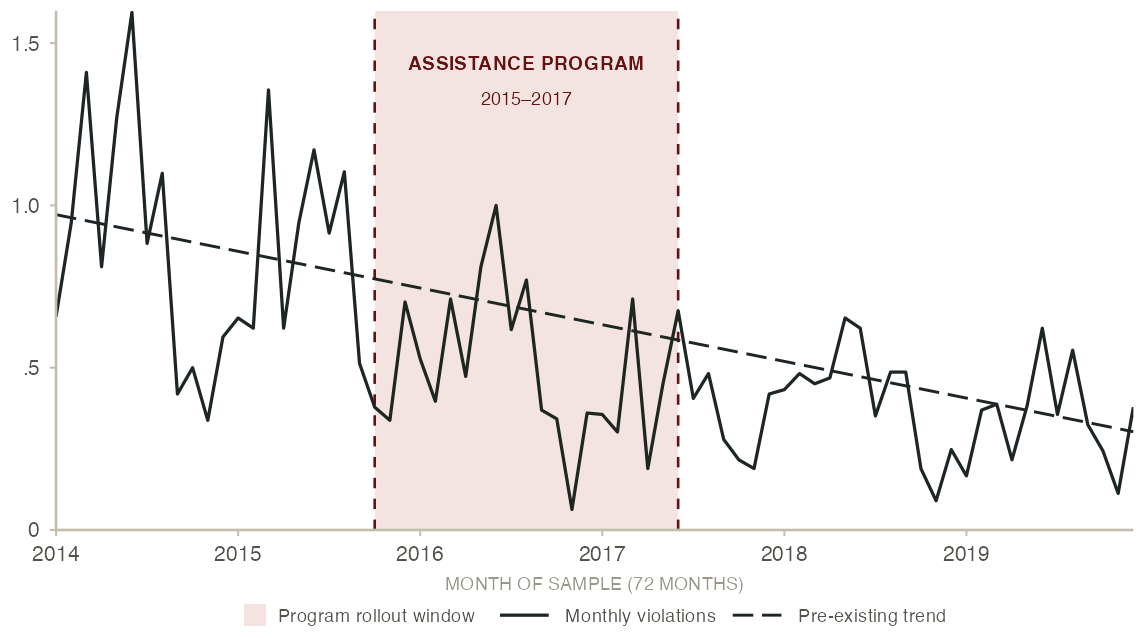
\includegraphics[width=\linewidth]{../figures/fig1.png}
\end{minipage}

\vspace{0pt}

% ---------------------------------------------------------------------
% IMPLICATIONS (ruled head) + THREE COLUMNS (11px body)
% ---------------------------------------------------------------------
\sectionhead{Implications}

\noindent
\begin{minipage}[t]{0.310\linewidth}
\colhead{Funding}
{\impcolsize Given scarce enforcement resources, programs need to actually work. This study indicates \brieflink{compliance assistance may not be as effective as previously thought}.\par}
\end{minipage}\hfill
\begin{minipage}[t]{0.310\linewidth}
\colhead{Alternatives}
{\impcolsize The \brieflink{trade-offs of different policies should be weighed as the EPA plans future programs}. Assistance is not proven to be as effective as inspections, though that is not to say they'll never be effective.\par}
\end{minipage}\hfill
\begin{minipage}[t]{0.310\linewidth}
\colhead{Oversight}
{\impcolsize The EPA does not systematically collect data on compliance assistance activities (GAO, 2020), and \brieflink{this study underscores the need for more deliberate program evaluation}.\par}
\end{minipage}

% ---------------------------------------------------------------------
% FOOTER (pinned to bottom)
% ---------------------------------------------------------------------
\brieffooter{Method: pre-registered difference-in-differences on monthly facility violation records. Full paper: doi.org/10.1002/pam.70056}




\end{document}
